\documentclass[12pt,a4paper]{article}
\usepackage{graphicx}
\usepackage{placeins}
\usepackage{indentfirst}
\usepackage{polski}
\usepackage[utf8]{inputenc}
\title{Sprawozdanie z laboratorium PAMSI}
\author{Damian Oleksak}
\date{}
\begin{document}
\maketitle
\newpage

\section*{Wstęp}

Graf jest strukturą składającą się ze zbioru wierzchołków oraz krawędzi. Z każdą krawędzią skojarzona jest para wierzchołków.
Każdej krawędzi przypisujemy wagę, która reprezentuje (w zastosowaniach praktycznych) np. długość drogi, koszt
budowy drogi, czas lub koszt przejazdu, niezawodność połączenia, prawdopodobieństwo przejścia, lub przepustowość. Przy implementacji grafu możemy posłużyć się macierzą wag lub listą krawędzi. Macierz wag to tablica 2-wymiarowa o rozmiarze
 $n\times n $, w której wartość na przecięciu i-tego wiersza i j -tej kolumny oznacza wagę krawędzi (i, j). W tym przypadku zajętość pamięci wynosi $ O(n^{2}) $ .
Połączone listy sąsiadów to struktura składająca się z tablicy n
list, gdzie lista dowiązana do komórki i-tej zawiera wszystkie krawędzie incydentne z wierzchołkiem i-tym (waga krawędzi i oznaczenie wierzchołka). Zajętość pamięci - O(n + m).


Przeszukiwanie grafu lub inaczej przechodzenie grafu to czynność polegająca na odwiedzeniu w jakiś usystematyzowany sposób wszystkich wierzchołków grafu w celu zebrania potrzebnych informacji. Powszechnie stosuje się dwie podstawowe metody przeszukiwania grafów:\newline
-przeszukiwanie wszerz;\newline
-przeszukiwanie w głąb.\newline
\newline
Gdy chcemy znaleźć najkrótszą ścieżkę w grafie ważonym z dowolnego wierzchołka do wierzchołka spełniającego określony warunek, możemy zastosować algorytm A*. Jest on stosowany głównie do rozwiązywania problemów w grach komputerowych, np gdy chcemy, by postać przemieściła się po planszy z pkt. A do pkt. B i zrobiła to w miarę inteligentny sposób.

\newpage

\section*{Przykład}

Weźmy za przykład poniższy graf:\newline

\begin{figure}[h]
\centering
\caption[Graf]{}
\label{fig:graf}
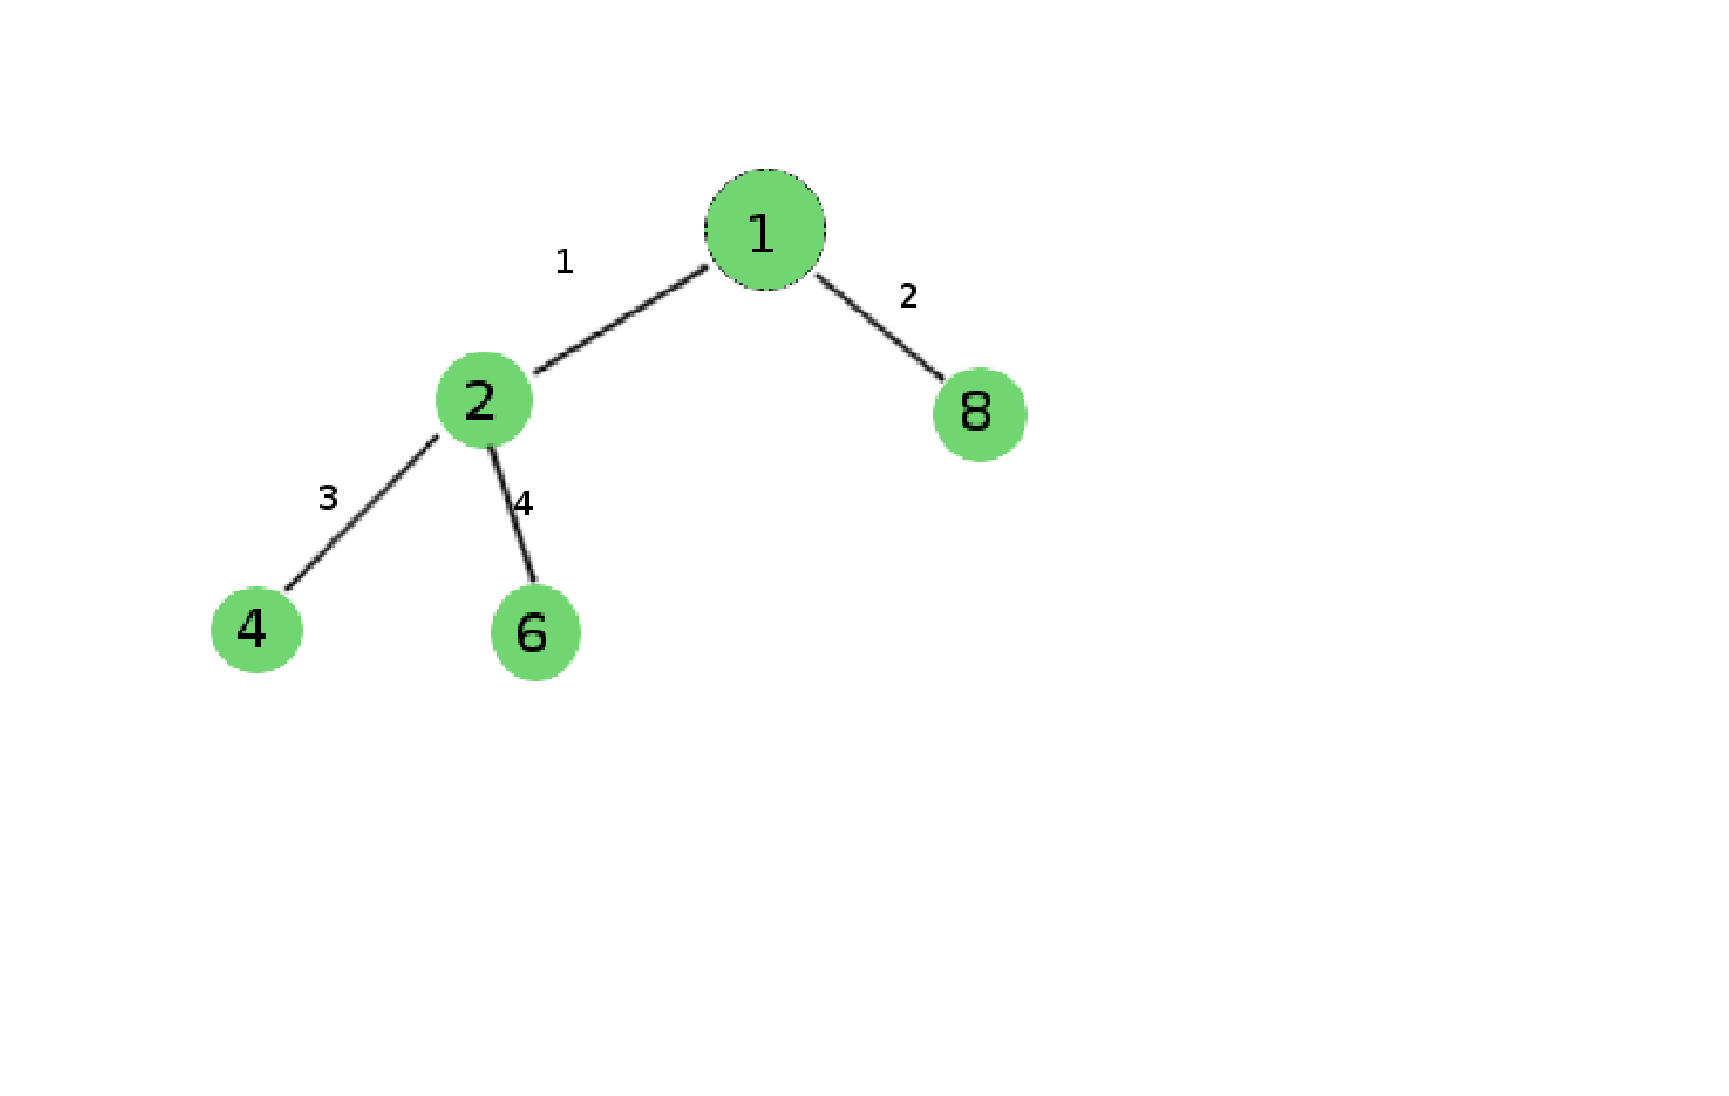
\includegraphics[width=0.7\linewidth]{./graf}
\end{figure}


Przeszukiwanie w głąb polega na badaniu wszystkich krawędzi wychodzących z podanego wierzchołka. Po zbadaniu wszystkich krawędzi wychodzących z danego wierzchołka algorytm powraca do wierzchołka, z którego dany wierzchołek został odwiedzony.\newline
$ 1 \mapsto 2 \mapsto 4 \mapsto 6 $  - ścieżka przeszukiwania DFS zrealizowana w programie.\newline
\newline
Przeszukiwanie wszerz rozpoczyna się od początkowego wierzchołka 1 i polega na odwiedzeniu wszystkich osiągalnych z niego wierzchołków.\newline
$ 1 \mapsto 2 \mapsto 8 \mapsto 4 \mapsto 6 $ - ścieżka przeszukiwania BFS zrealizowana w programie. \newline


Algorytm A* rozpoczyna od punktu startowego 1 i rozpoczyna poszukiwania do momentu odnalezienia celu - wierzchołek 6.
Rozpoczynamy poszukiwania postępując zgodnie z następującymi punktami:\newline

1. Zaczynamy w punkcie startowym A i dodajemy go do "Listy Otwartych" - pól oczekujących na sprawdzenie. Lista Otwartych zawiera pola które mogą zawierać się w poszukiwanej ścieżce (pola, które wymagają sprawdzenia).\newline

2. Szukamy wszystkich osiągalnych pól, przyległych do pola startowego (pkt. A). Dodajemy je do Listy Otwartych. Dla każdego z tych pól zachowujemy pkt. A jako "pole rodzica".\newline

3. Usuwamy pole startowe A z Lisy Otwartych i dodajemy je do Lisy Zamkniętych, by zaznaczyć, że nie musimy sprawdzać go ponownie.\newline
\newline
Wybór pól wyznaczających poszukiwaną ścieżkę, determinuje poniższe równanie:\newline

F = G + H\newline 

gdzie:\newline

    G = koszt ruchu z punktu startu A do aktualnej pozycji, potrzebny by podążając wyznaczoną dotychczas ścieżką osiągnąć aktualną pozycję. \newline
    H = szacunkowy koszt ruchu przejścia z aktualnej pozycji do celu wędrówki (pkt. B). Jest często określany jako heurystyka. Sposobem wyznaczania H jest szacowanie, ponieważ nie znamy aktualnego dystansu do momentu odnalezienia ścieżki. H może być wyznaczone na wiele sposobów. Najczęściej spotyka się metodę Manhattan. Polega ona na obliczeniu całkowitej ilości pól koniecznych do przejścia od aktualnej pozycji do celu (pkt. B). Następnie wynik mnożymy przez szacunkowy koszt jednego kroku. Nazwa metody (prawdopodobnie) pochodzi od miejskiego sposobu obliczania liczby bloków między jednym miejscem a drugim, kiedy nie można przeciąć bloku na skos.\newline

Nasza ścieżka jest generowana przez powtarzanie przeglądania Listy Otwartych i wybieranie spośród jej zawartości pól o najniższym koszcie F. \newline

$ 1 \mapsto 2 \mapsto 8 \mapsto 4 \mapsto 6 $ - ścieżka przeszukiwania A* zrealizowana w programie. \newline

\section*{Uwagi i wnioski}
Algorytm A* nie zawsze musi być szybszy od trawersacji grafu wszerz czy w głąb. Zależy to od struktury badanego grafu. W naszym przypadku A* odwiedził wszystkie wierzchołki i zajęło mu to 264 mikrosekund.

\end{document} 
